\chapter{Results}
\label{chap:Results}



\section{Touschek Studies}

\subsection{HER}

	Touschek effect not obvious in HER data.


\begin{figure}[htb]
	\centerfloat
		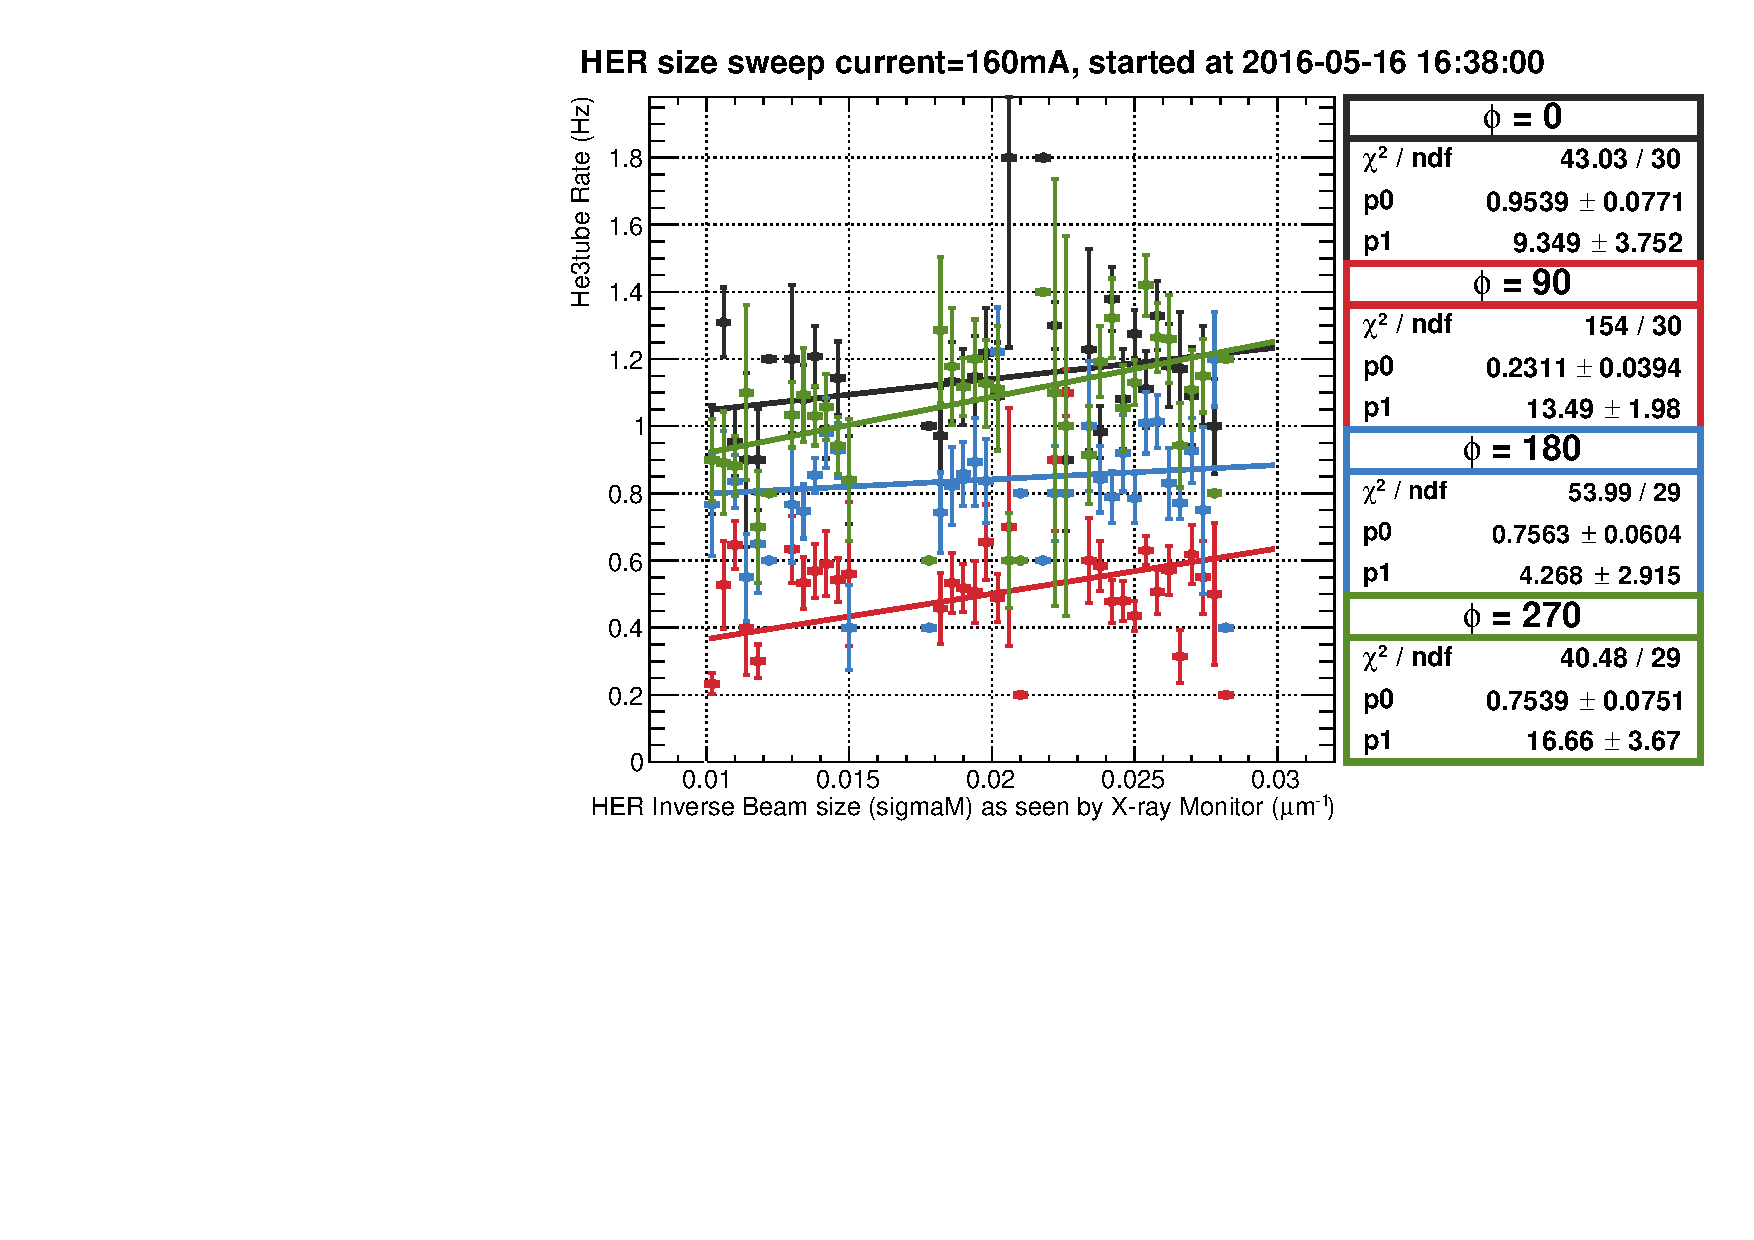
\includegraphics[trim={0 0 0 0.75cm},clip, scale=0.6]{images/2006}
	\caption{Rate in Helium-3 tubes vs HER inverse beam size at a current of 160mA}	
	\label{fig:TousHER2006}
\end{figure}

\begin{figure}[htb]
	\centerfloat
		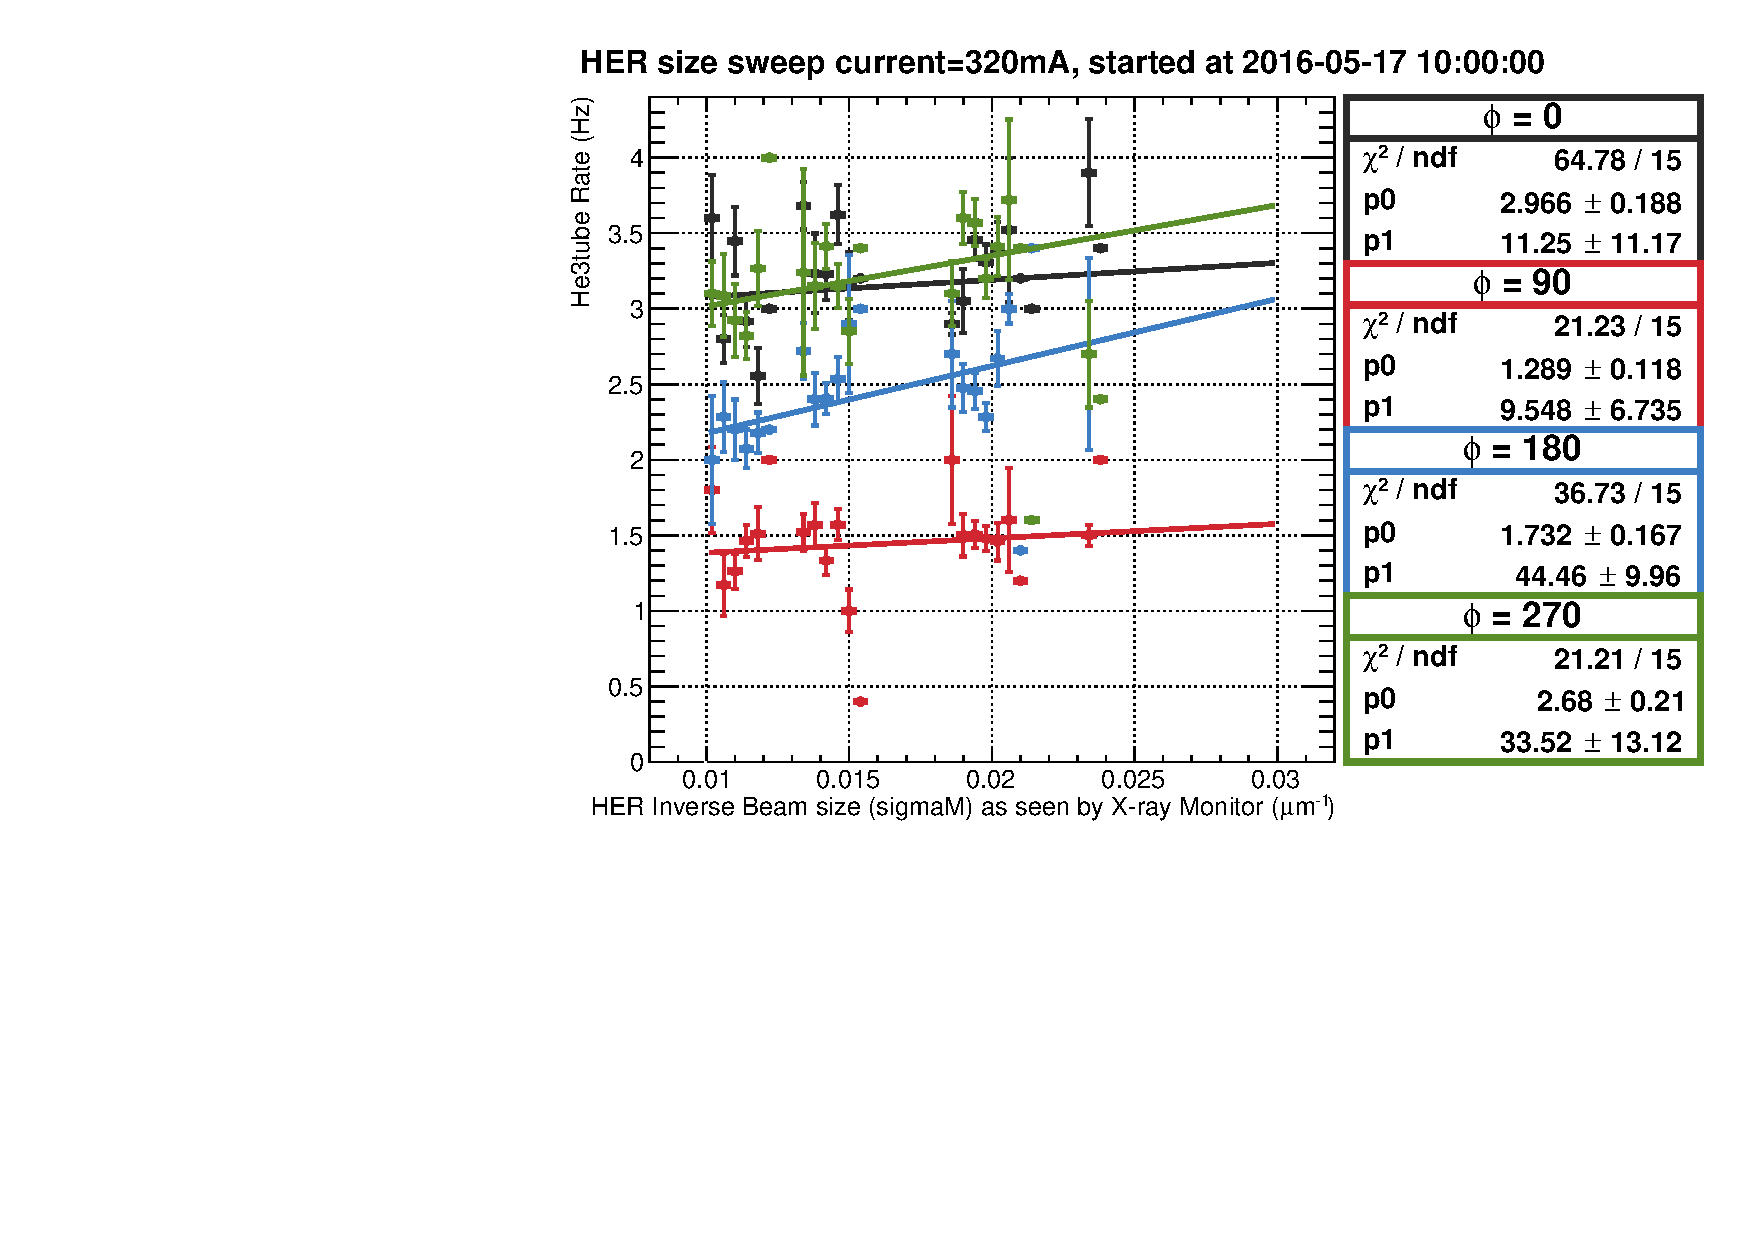
\includegraphics[trim={0 0 0 0.75cm},clip, scale=0.6]{images/2007}
	\caption{Rate in Helium-3 tubes vs HER inverse beam size at a current of 320mA}	
	\label{fig:TousHER2007}
\end{figure}

\begin{figure}[htb]
	\centerfloat
		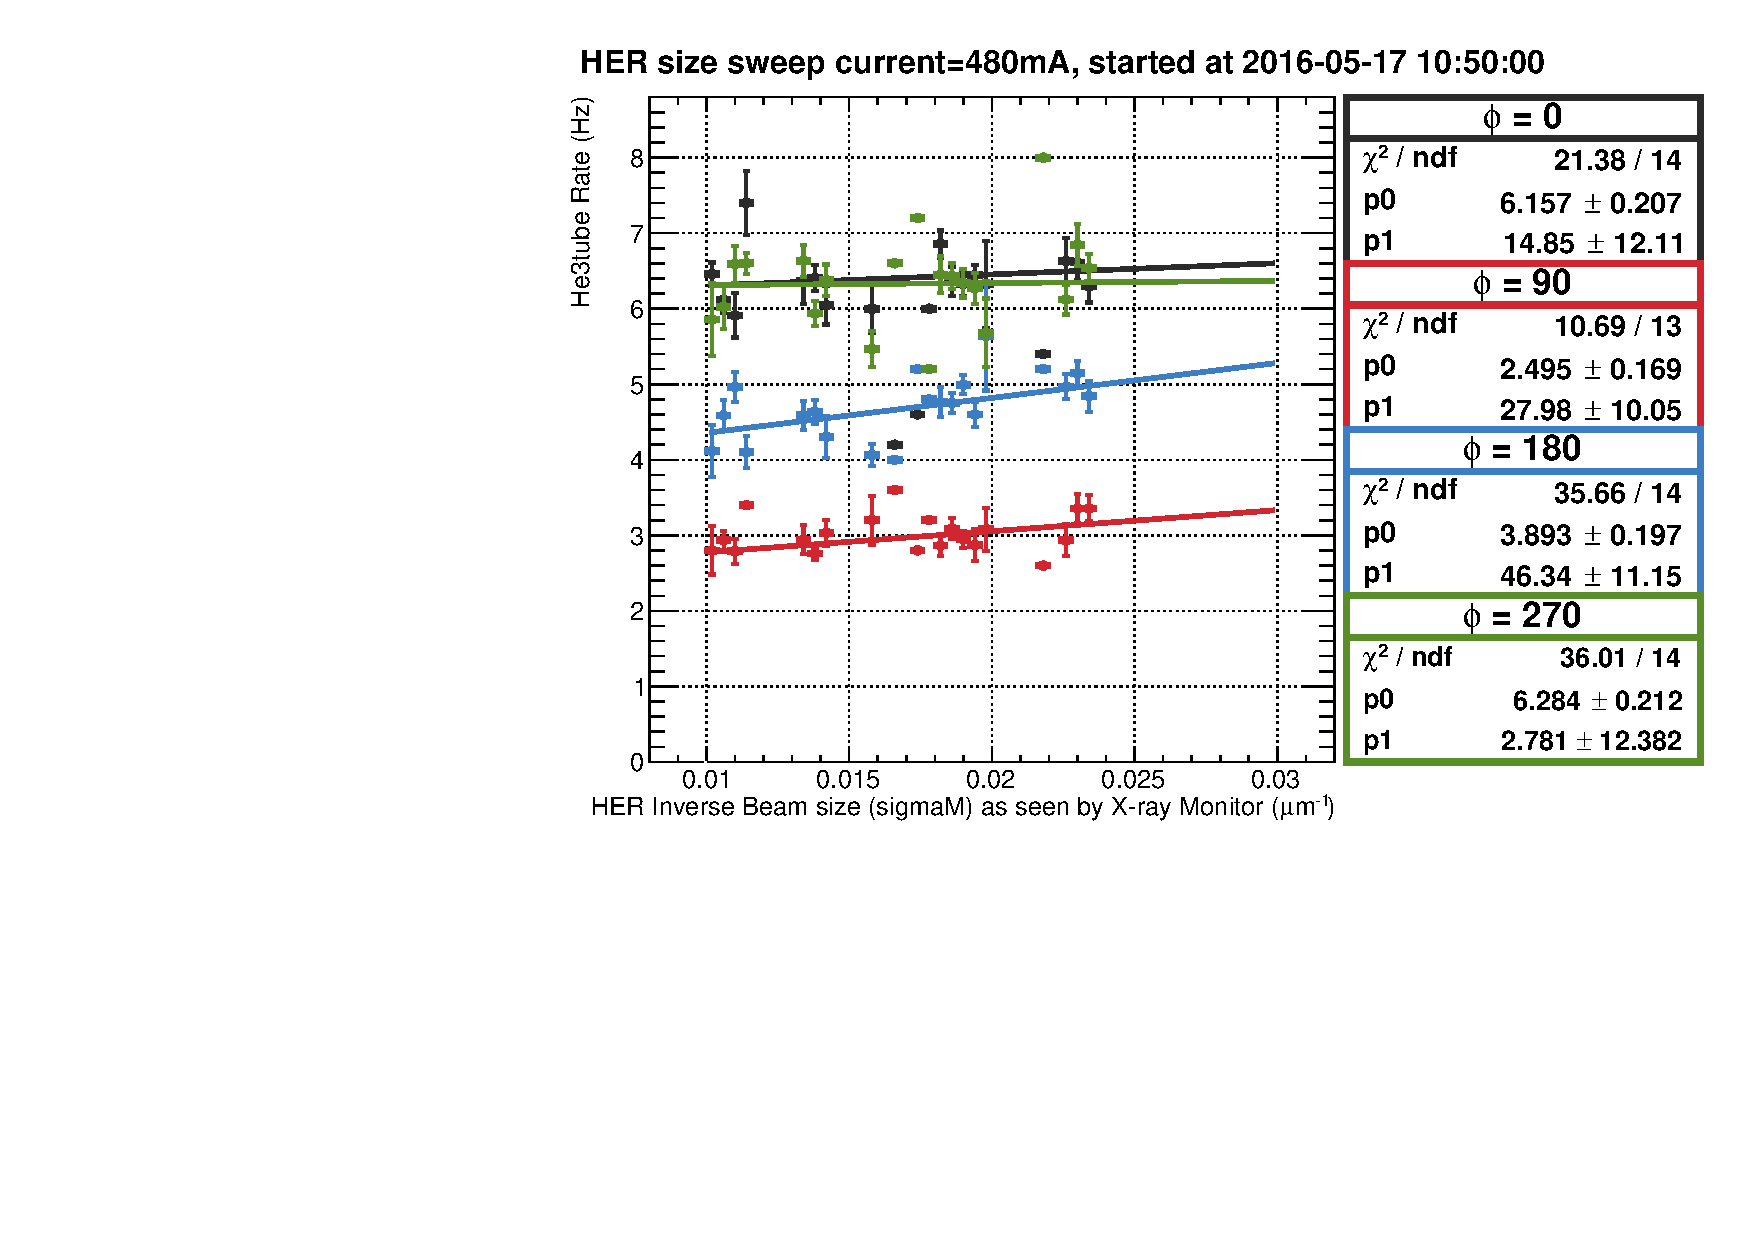
\includegraphics[trim={0 0 0 0.75cm},clip, scale=0.6]{images/2008}
	\caption{Rate in Helium-3 tubes vs HER inverse beam size at a current of 480mA}	
	\label{fig:TousHER2008}
\end{figure}

\begin{figure}[htb]
	\centerfloat
		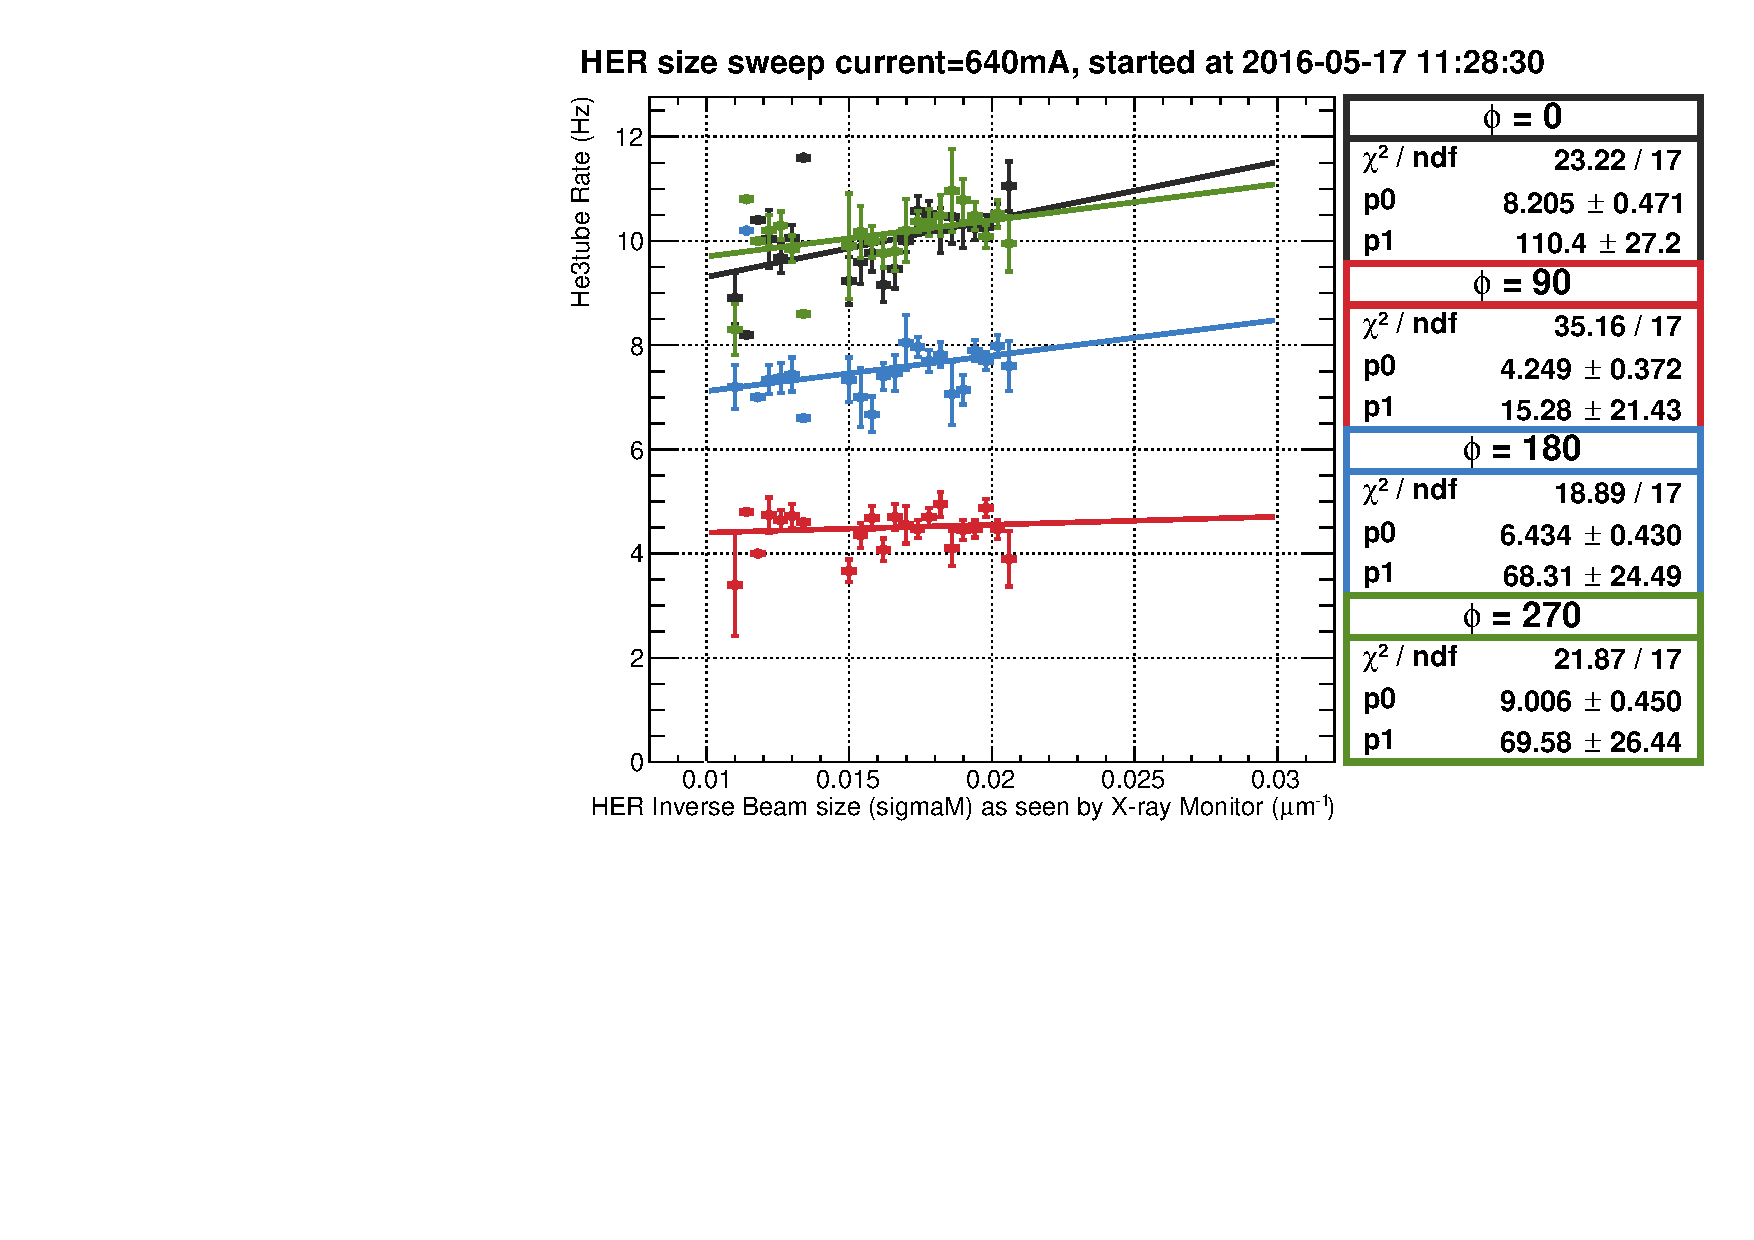
\includegraphics[trim={0 0 0 0.75cm},clip, scale=0.6]{images/2009}
	\caption{Rate in Helium-3 tubes vs HER inverse beam size at a current of 640mA}	
	\label{fig:TousHER2009}
\end{figure}

\begin{figure}[htb]
	\centerfloat
		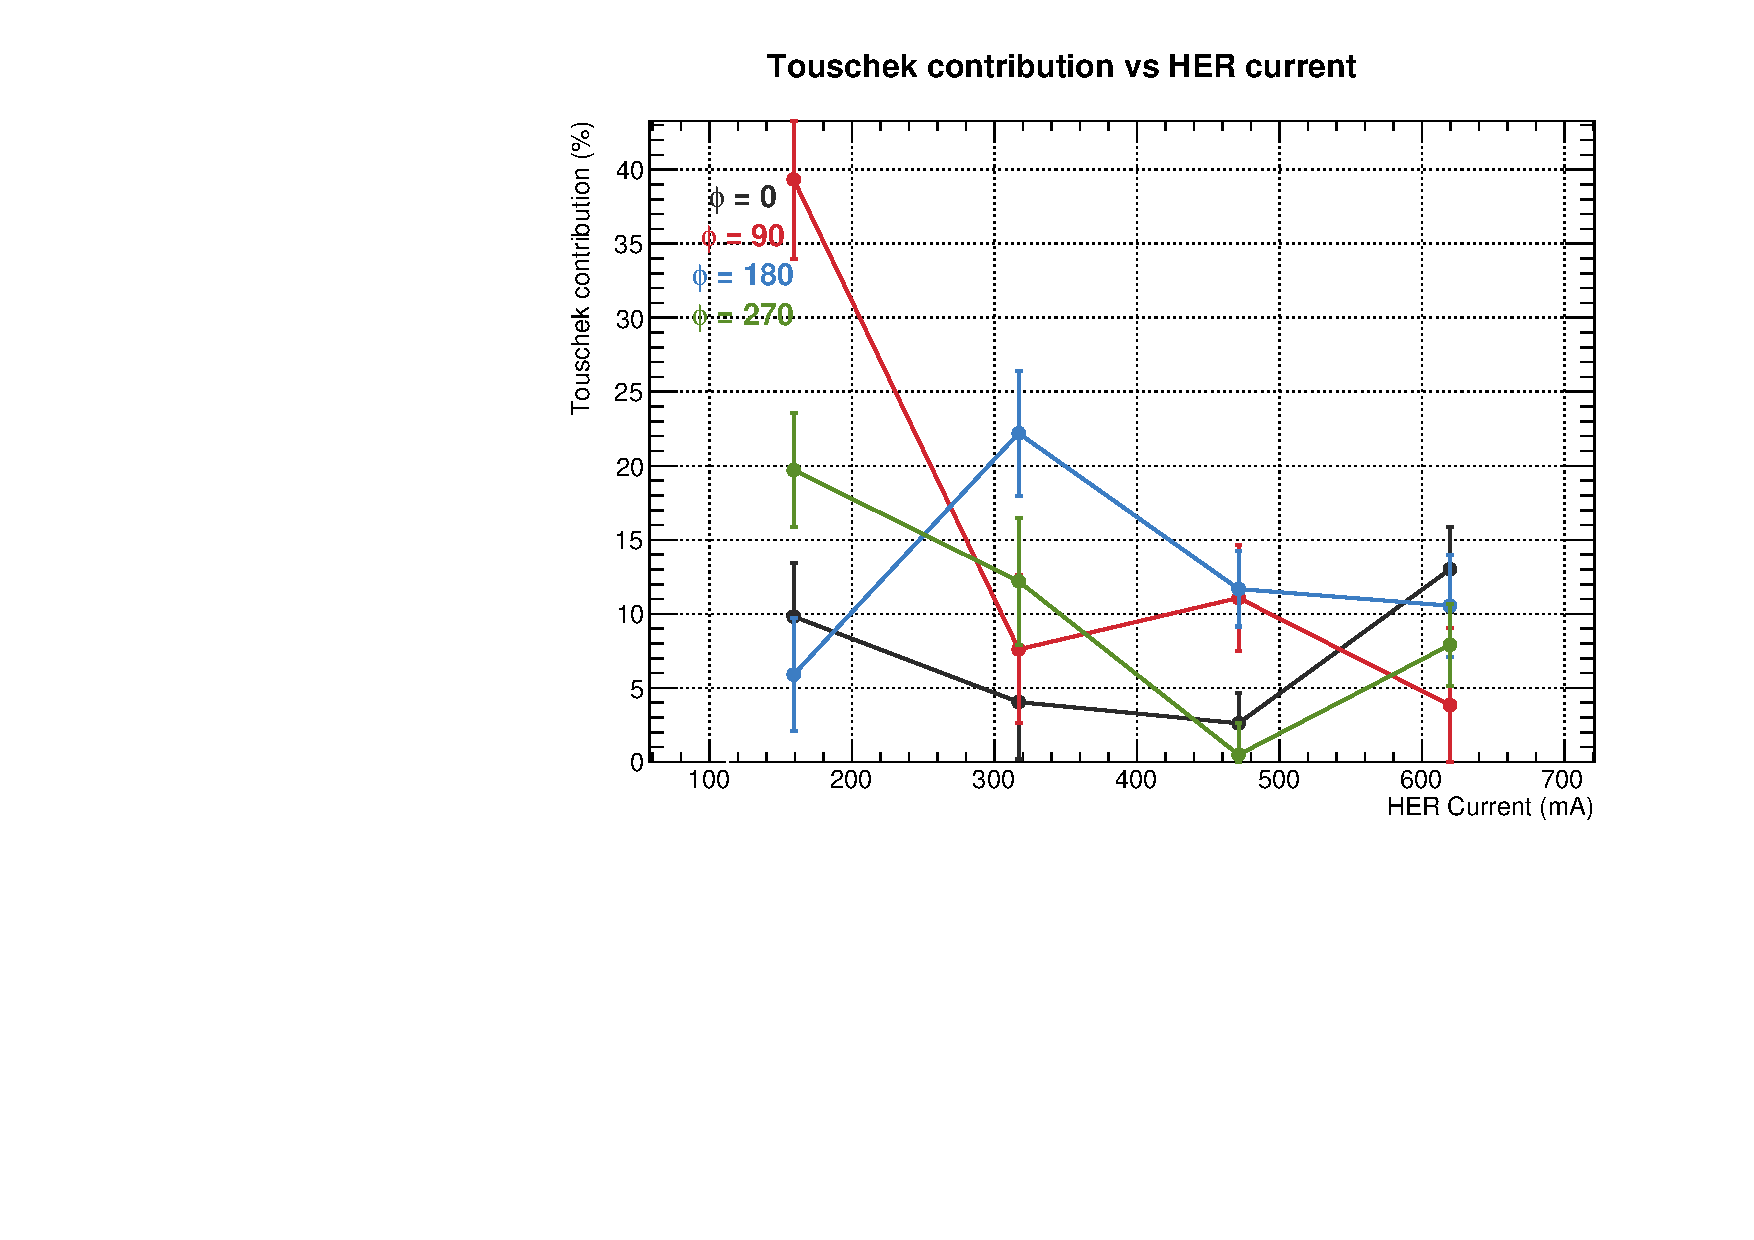
\includegraphics[scale=0.6]{images/HER_beamSize}
	\caption{HER Touschek contribution}	
	\label{fig:TousHERContrib}
\end{figure}

\clearpage

\subsection{LER}

\begin{figure}[htb]
	\centerfloat
		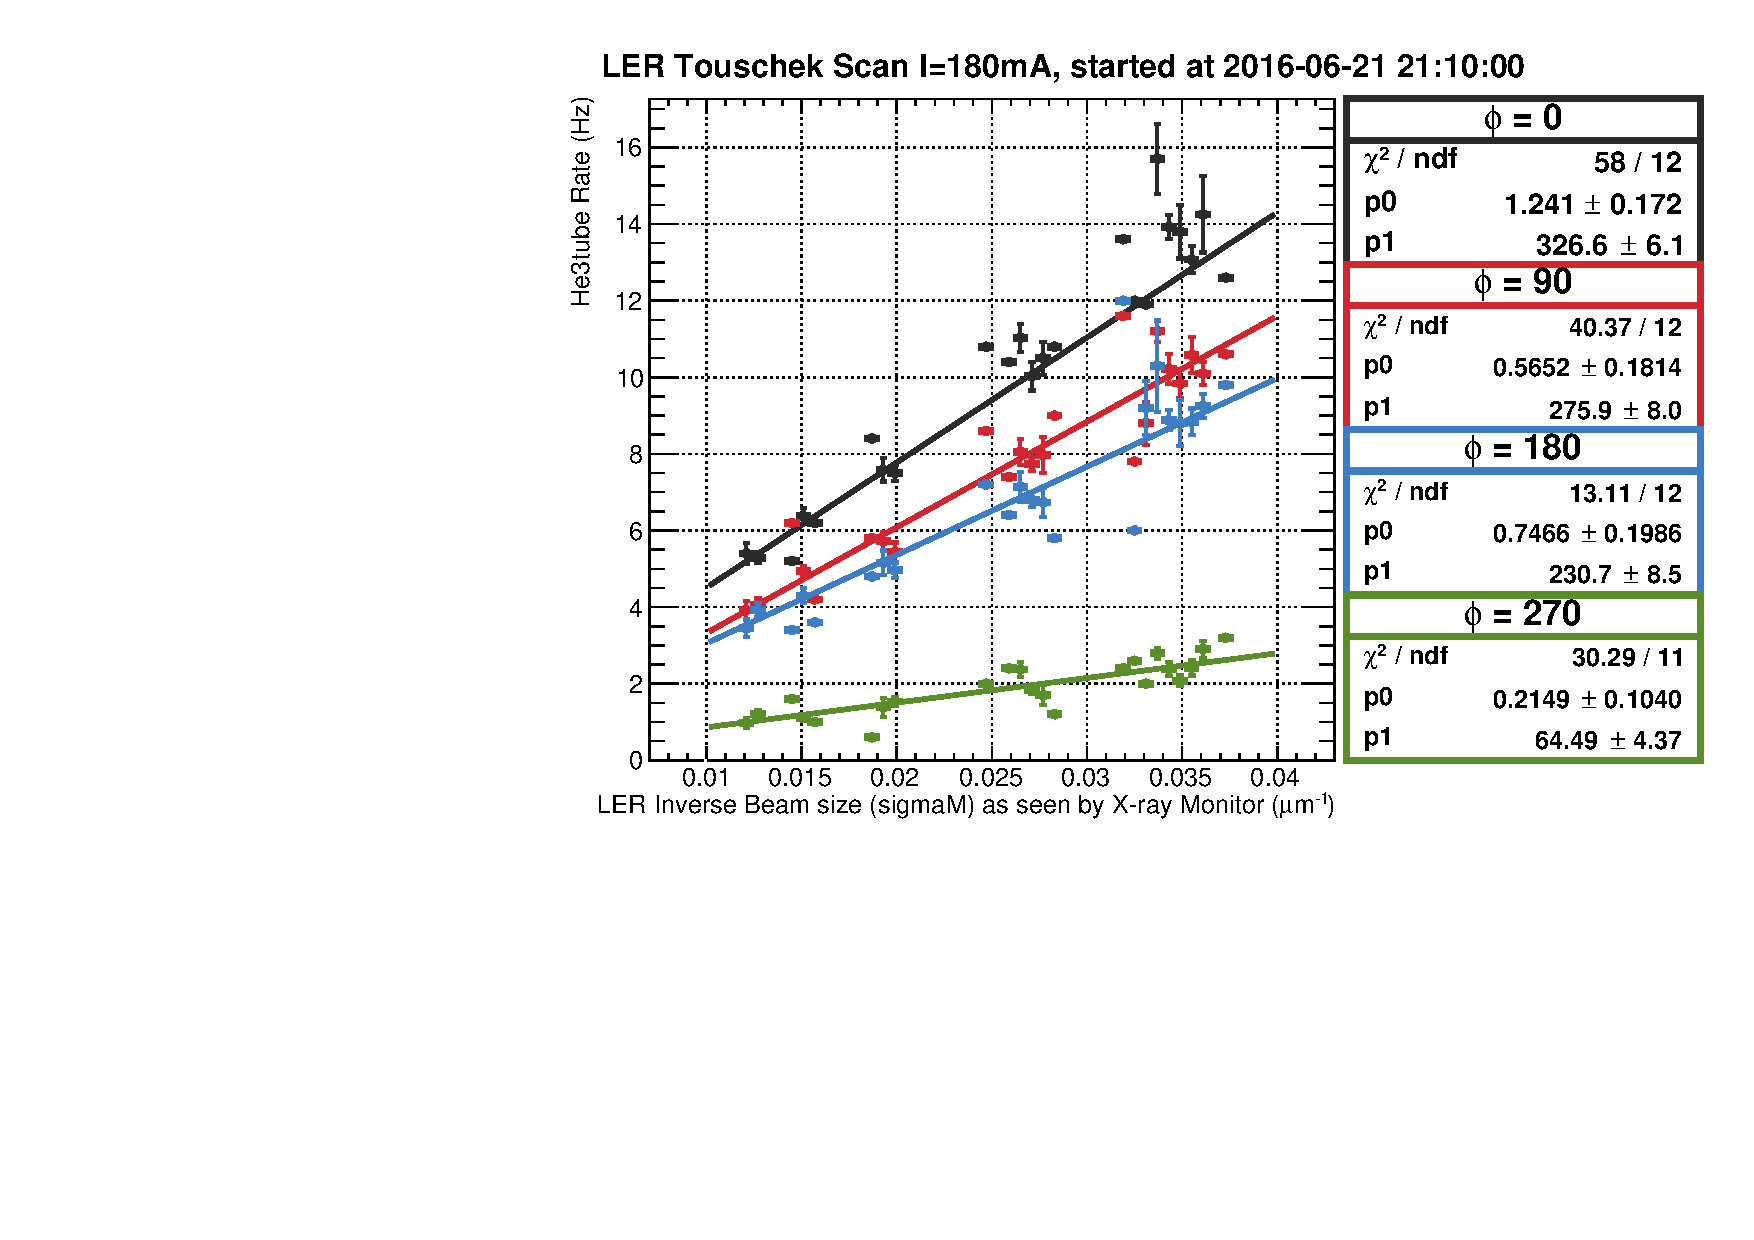
\includegraphics[trim={0 0 0 0.75cm},clip, scale=0.6]{images/12009}
	\caption{Rate in Helium-3 tubes vs LER inverse beam size at a current of 180mA}	
	\label{fig:TousLER12009}
\end{figure}

\begin{figure}[htb]
	\centerfloat
		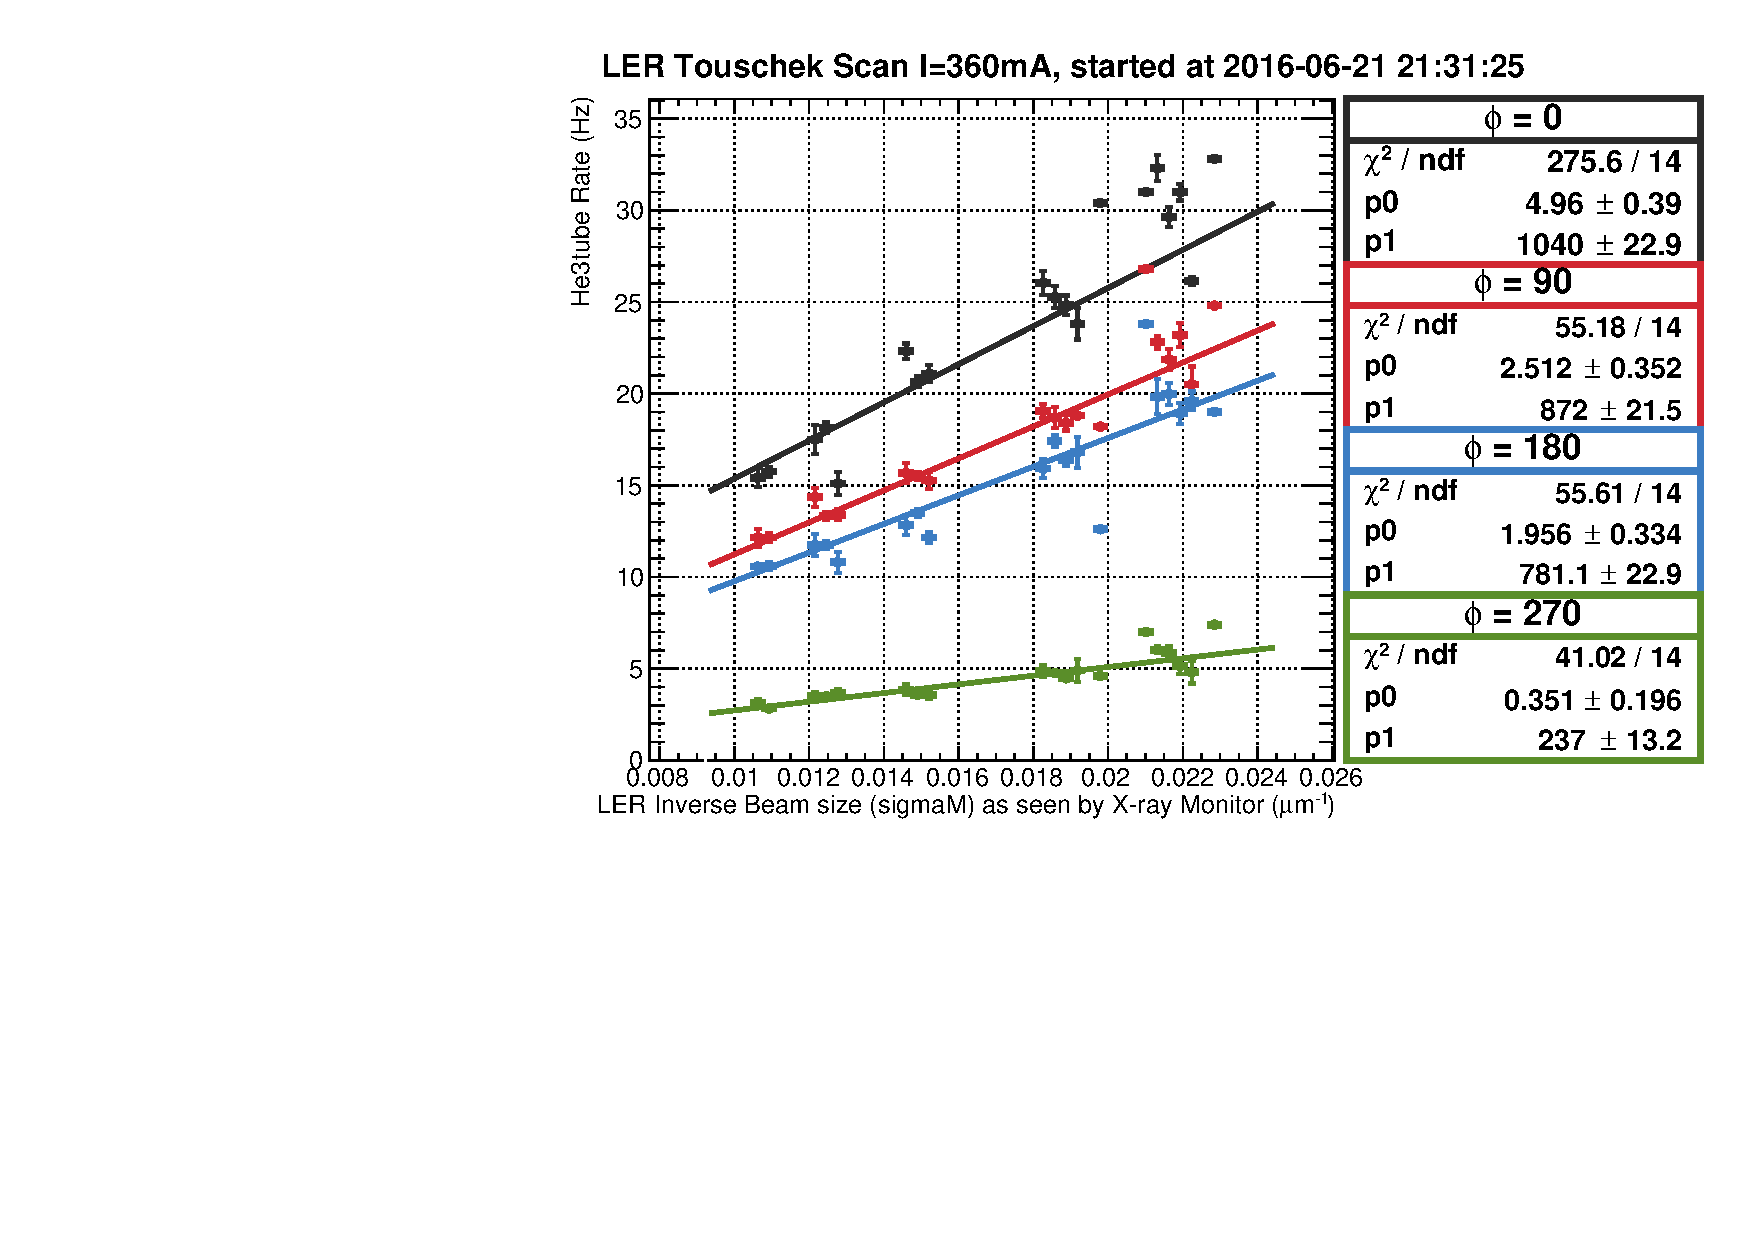
\includegraphics[trim={0 0 0 0.75cm},clip, scale=0.6]{images/13006}
	\caption{Rate in Helium-3 tubes vs LER inverse beam size at a current of 360mA}	
	\label{fig:TousLER13006}
\end{figure}

\begin{figure}[htb]
	\centerfloat
		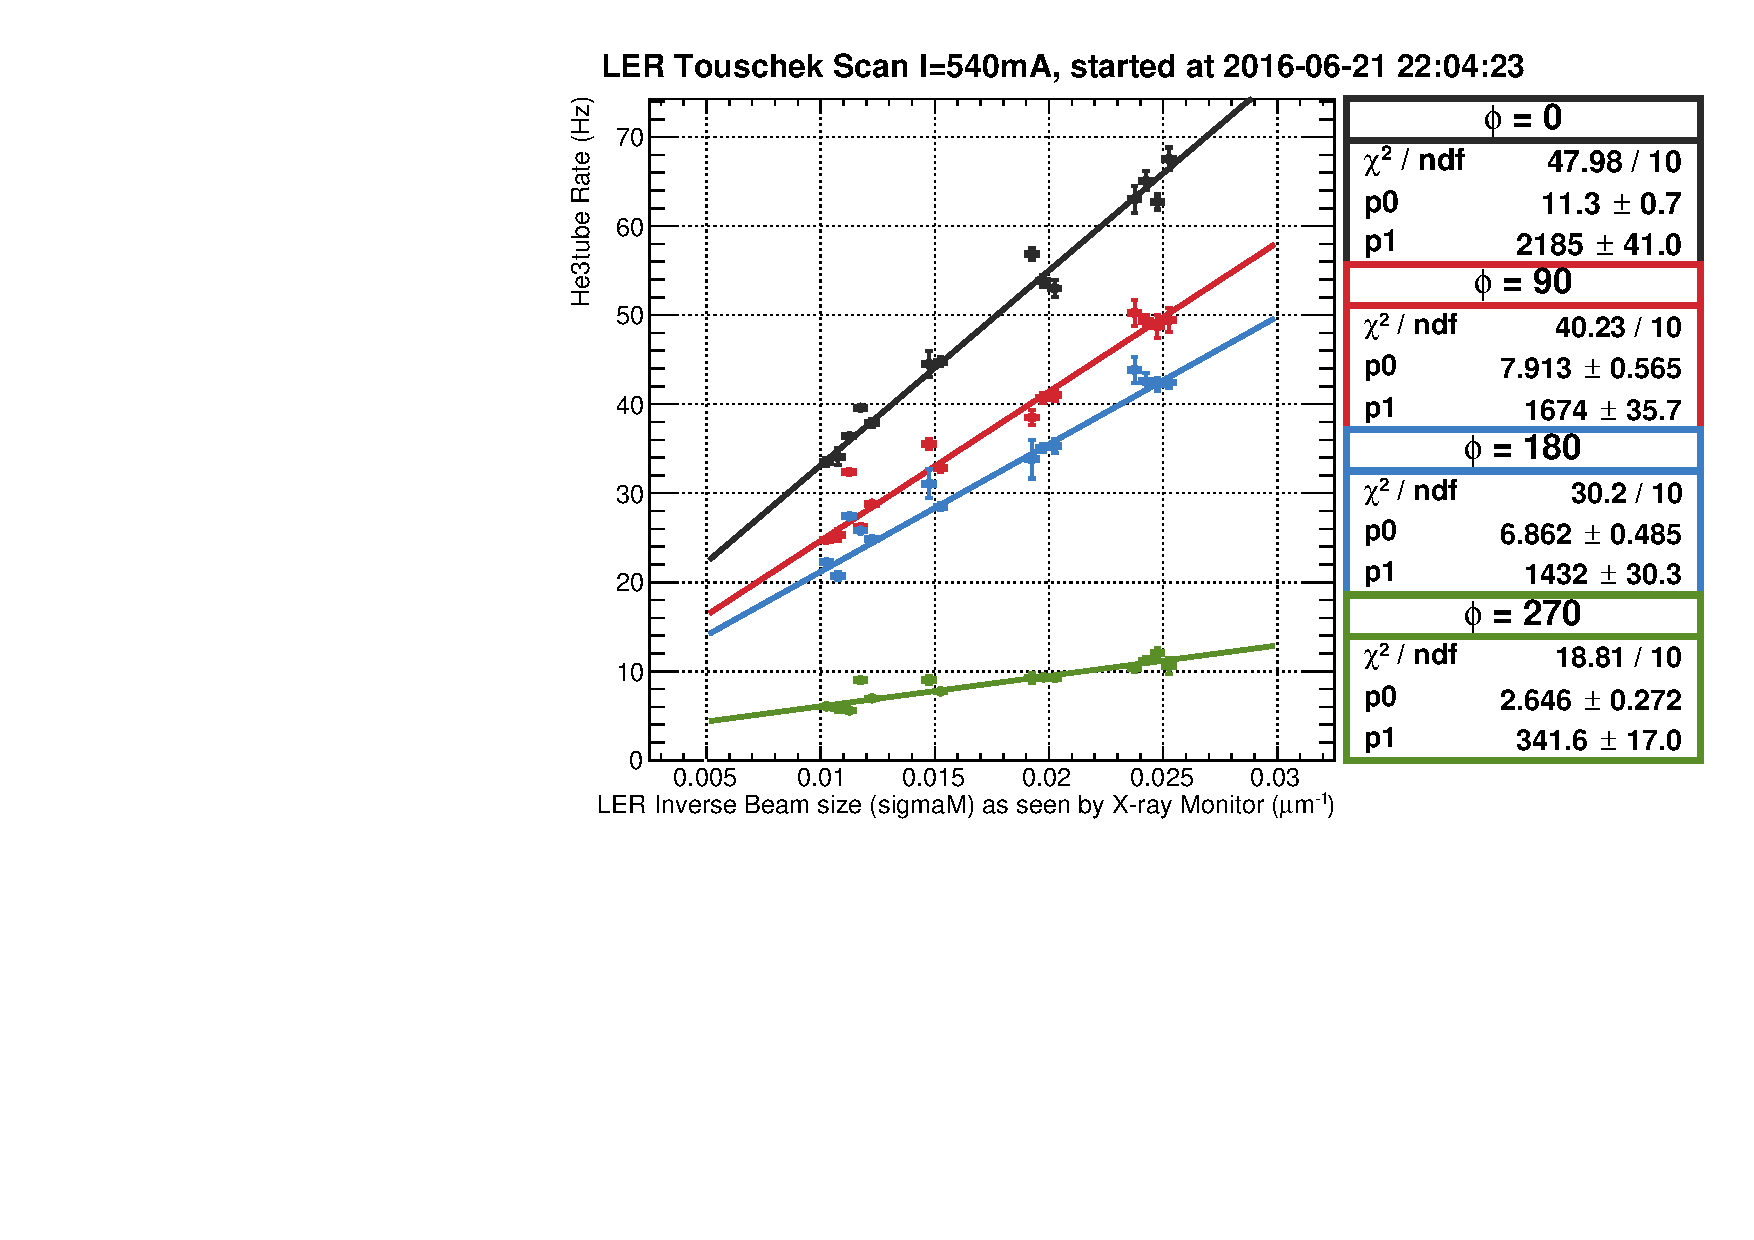
\includegraphics[trim={0 0 0 0.75cm},clip, scale=0.6]{images/13007}
	\caption{Rate in Helium-3 tubes vs LER inverse beam size at a current of 540mA}	
	\label{fig:TousLER13007}
\end{figure}


\begin{figure}[htb]
	\centerfloat
		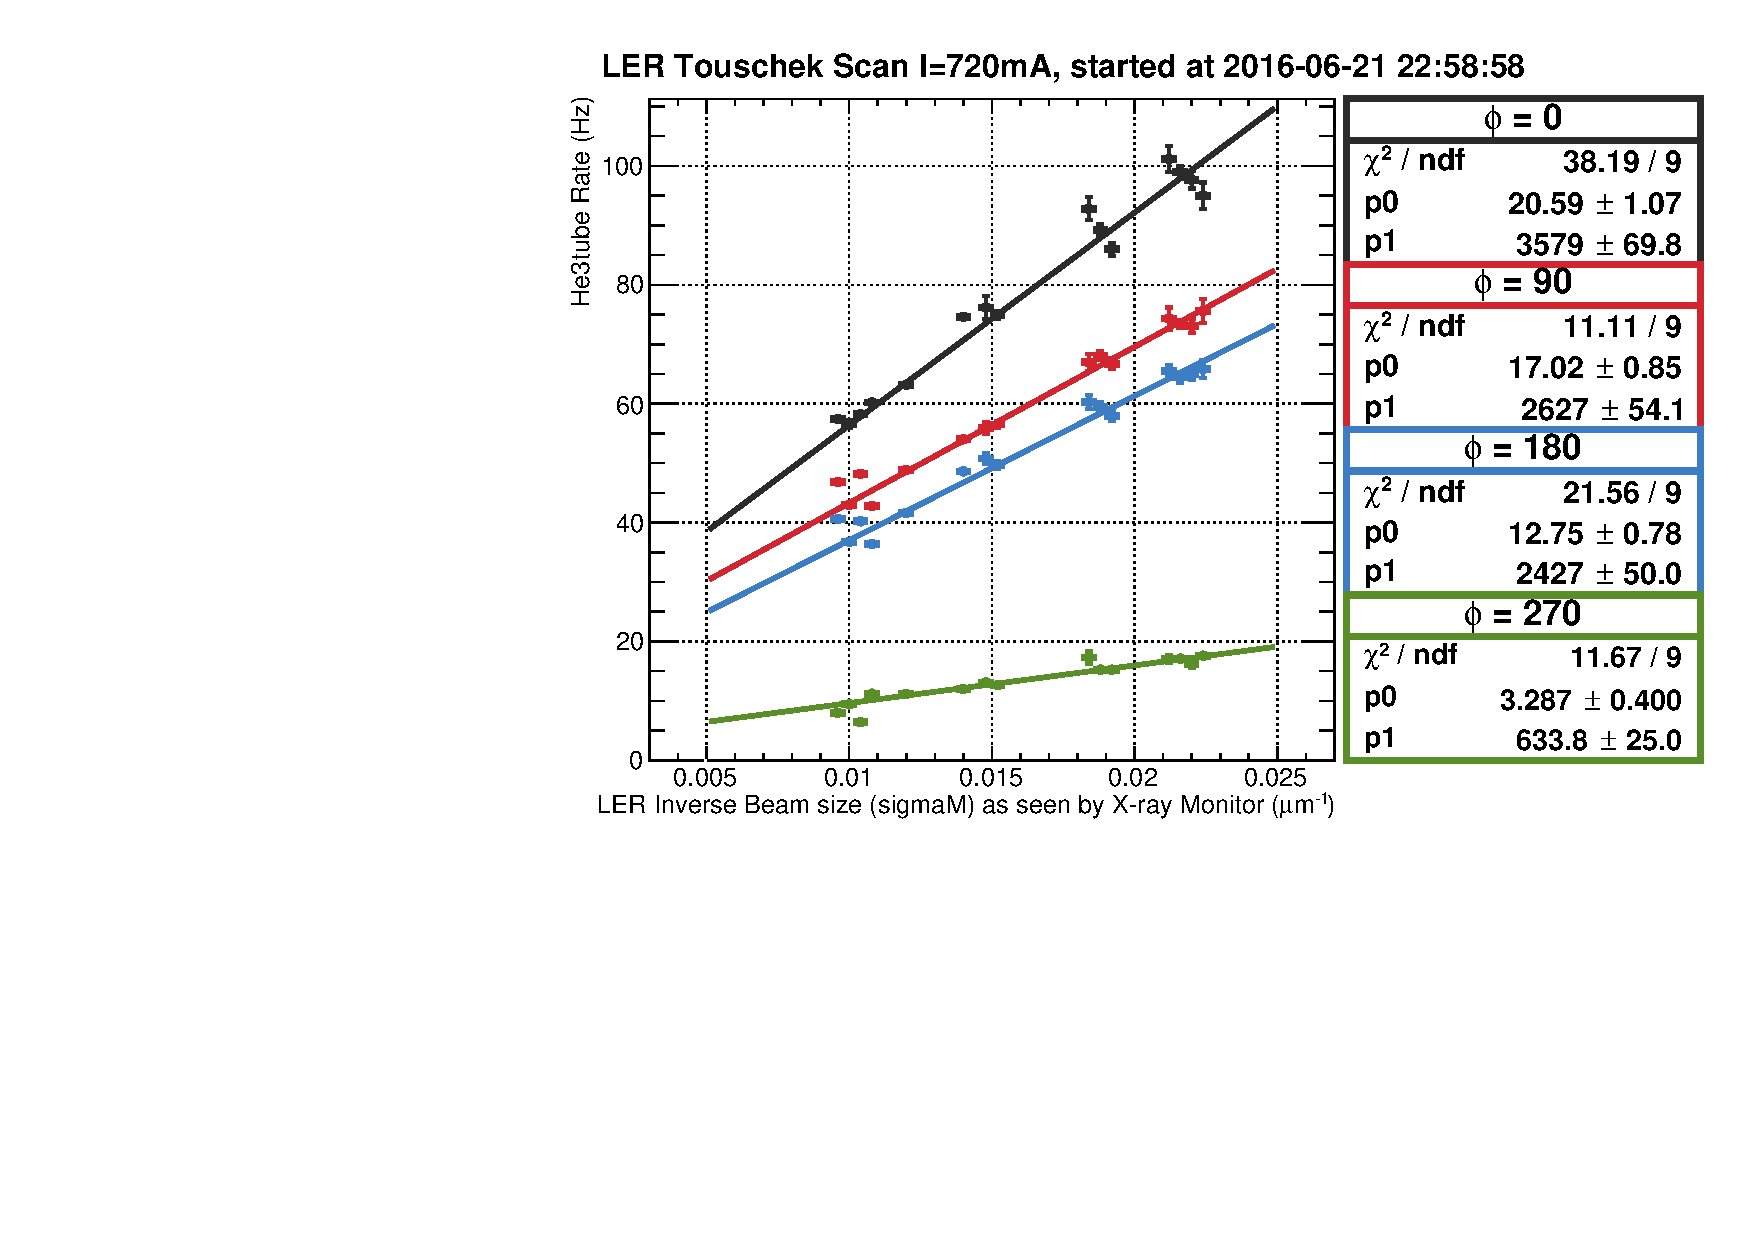
\includegraphics[trim={0 0 0 0.75cm},clip, scale=0.6]{images/13008}
	\caption{Rate in Helium-3 tubes vs LER inverse beam size at a current of 720mA}	
	\label{fig:TousLER13008}
\end{figure}


\begin{figure}[htb]
	\centerfloat
		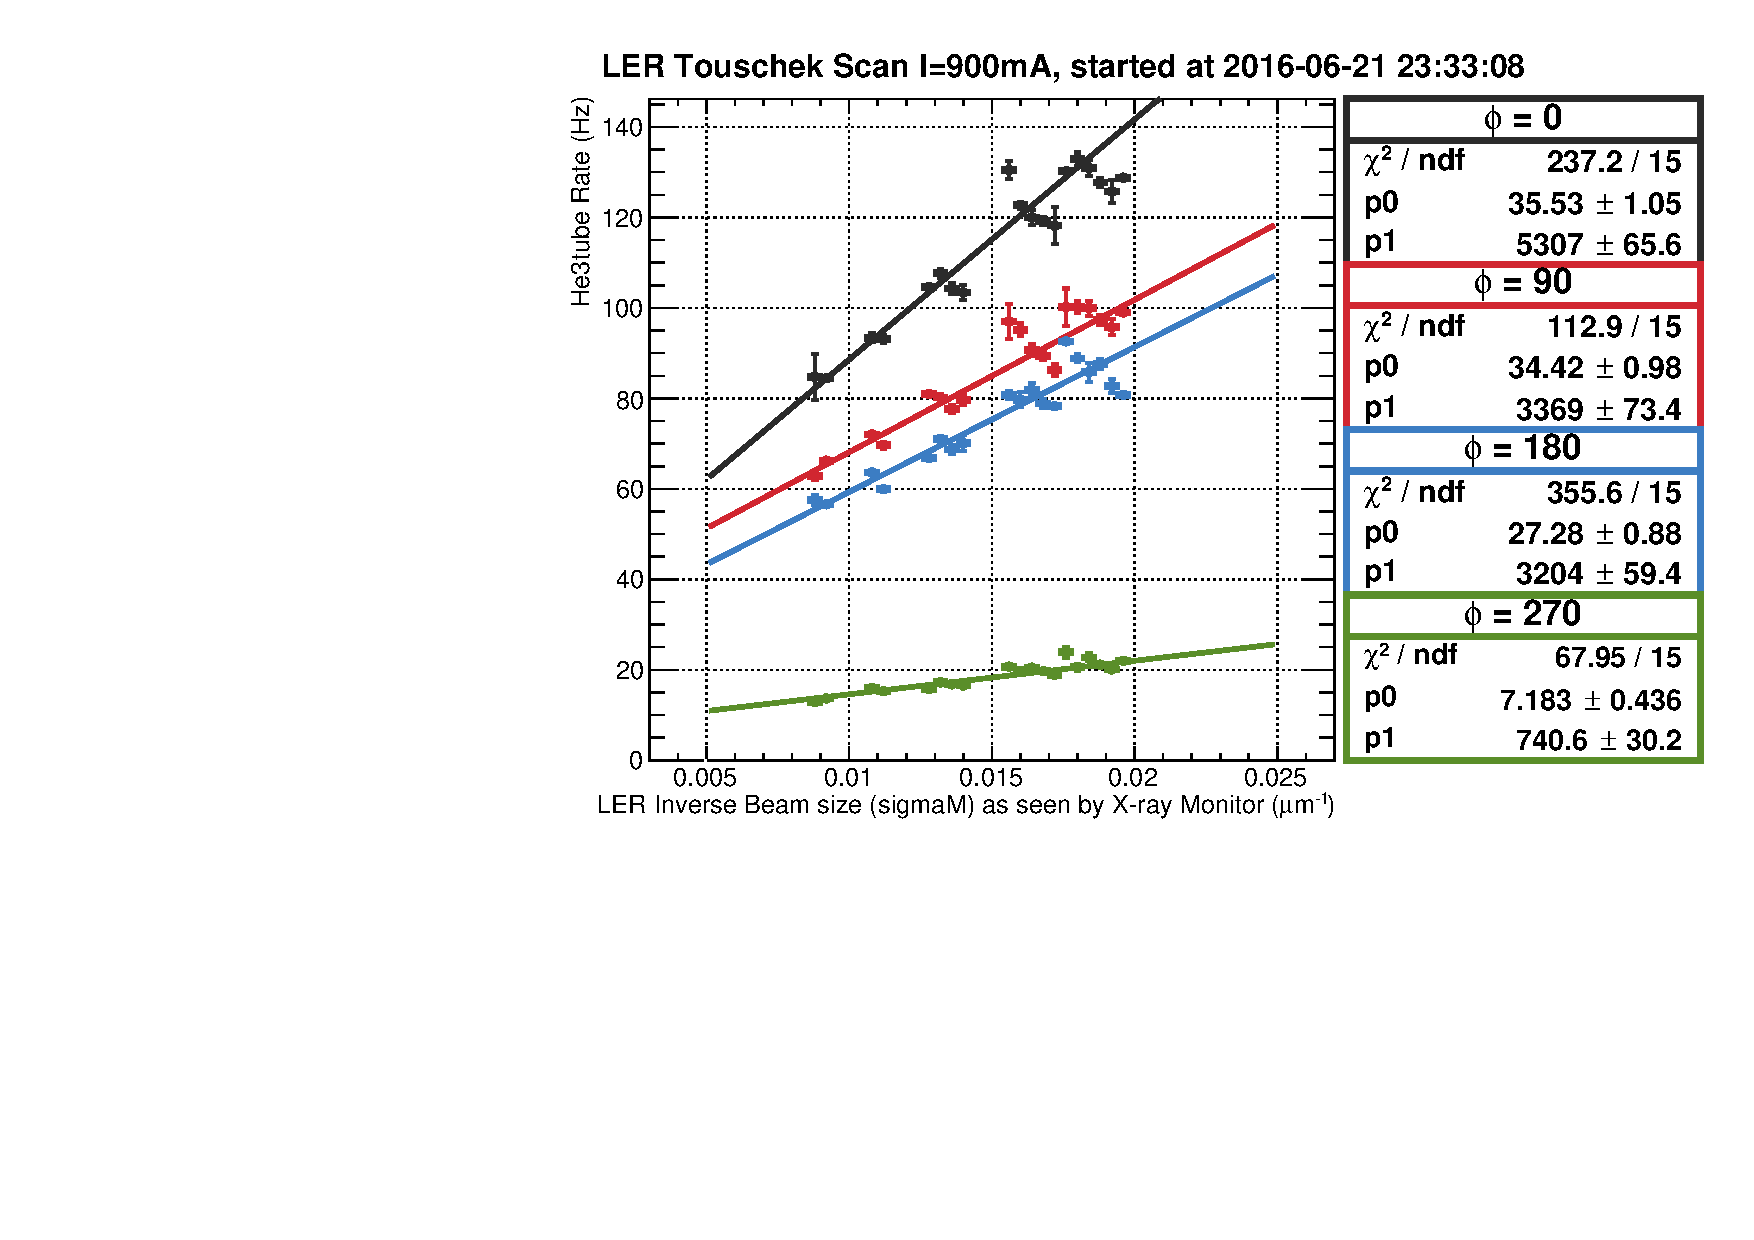
\includegraphics[trim={0 0 0 0.75cm},clip, scale=0.6]{images/13009}
	\caption{Rate in Helium-3 tubes vs LER inverse beam size at a current of 900mA}	
	\label{fig:TousLER13009}
\end{figure}


\begin{figure}[htb]
	\centerfloat
		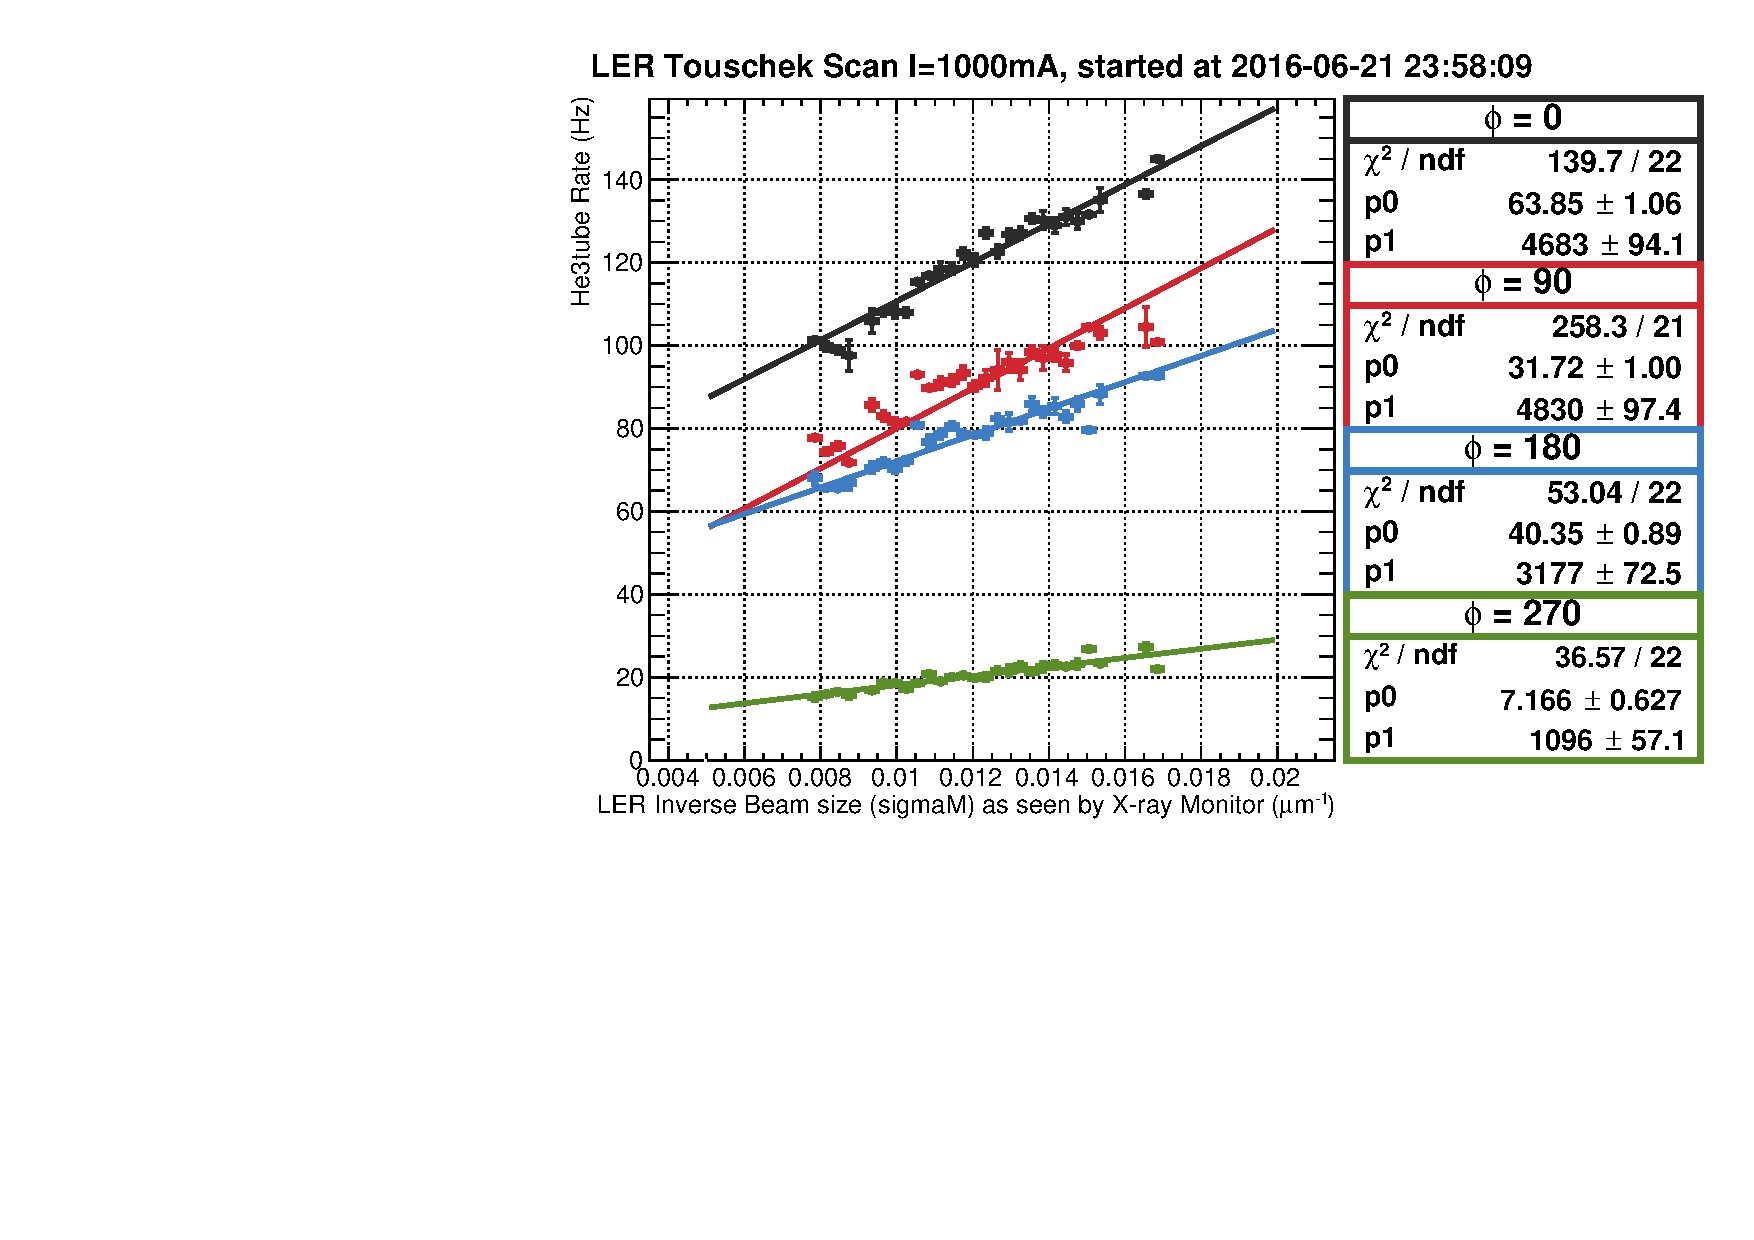
\includegraphics[trim={0 0 0 0.75cm},clip, scale=0.6]{images/13010}
	\caption{Rate in Helium-3 tubes vs LER inverse beam size at a current of 1000mA}	
	\label{fig:TousLER13010}
\end{figure}

\begin{figure}[htb]
	\centerfloat
		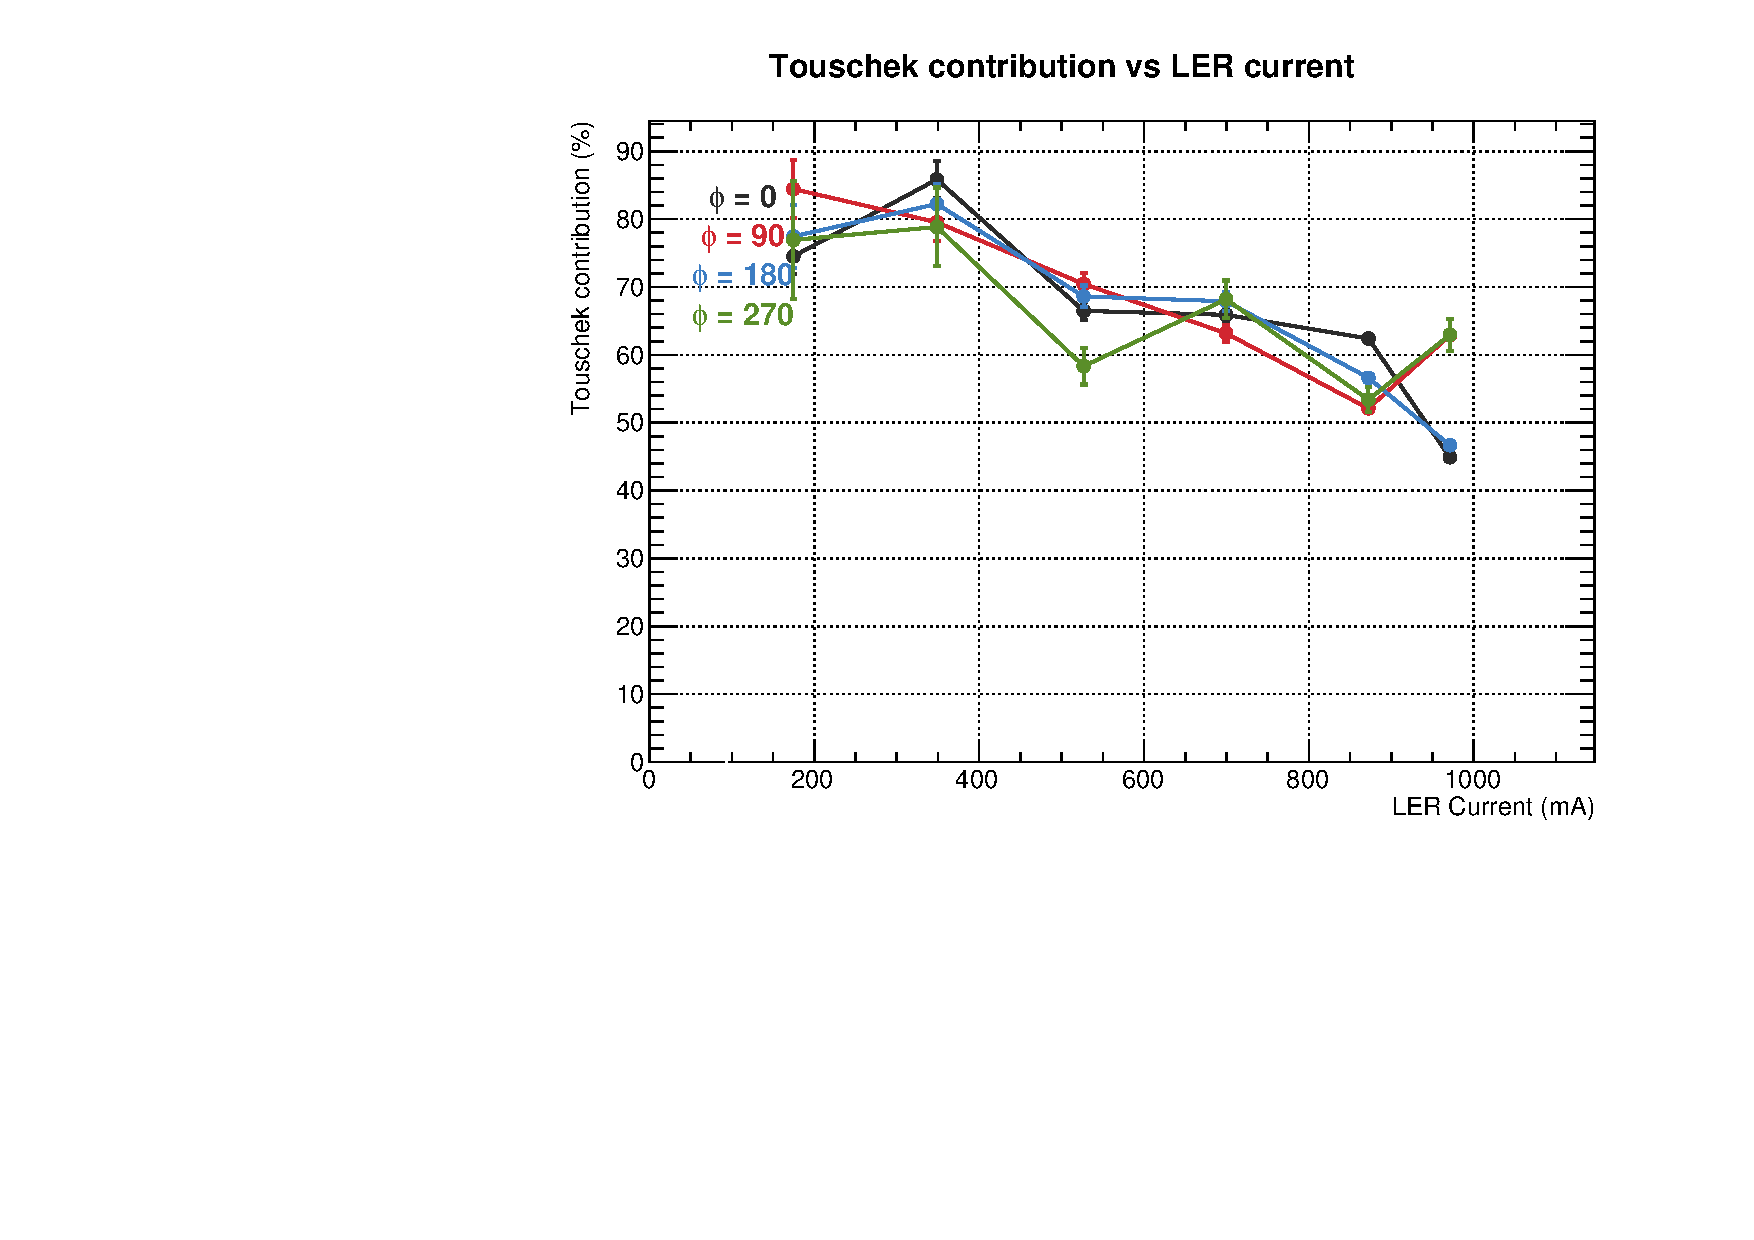
\includegraphics[scale=0.6]{images/LER_beamSize2}
	\caption{LER Touschek contribution}	
	\label{fig:TousLERContrib}
\end{figure}


\clearpage

\section{Vacuum Bump Studies}



\subsection{HER}

	No RGA data for HER.
	Is the double bump observed?

\subsection{LER}

	only have RGA data for run 5002.
	


